\documentclass[a4paper]{ltjsarticle}

\usepackage[dvipdfmx]{graphicx}
\usepackage[dvipdfmx,hidelinks,pdfusetitle]{hyperref}
\hypersetup{
    colorlinks=false,
    bookmarksnumbered=true,
    pdfborder={0 0 0},
    bookmarkstype=toc
}
\usepackage[nobreak]{cite}
\usepackage{pxjahyper}
\usepackage{amsmath}
\usepackage{tikz}

\usetikzlibrary{datavisualization}
\usetikzlibrary{positioning}
\usetikzlibrary{shapes.geometric, shapes.misc}
\usetikzlibrary{patterns}
\usetikzlibrary{calc}

\begin{document}

% ====================

\begin{itembox}[l]{東京工業大学 1984年}
    $n$ を3以上の整数とする.条件

    \begin{equation*}
        x+y+z=n,\ x\leqq y+z,\ y\leqq z+x,\ z\leqq x+y
    \end{equation*}

    を満たす正の整数の組 $(x,\ y,\ z)$ の個数を求めよ.
\end{itembox}

\begin{align}
    x+y+z & =n,\ x\leqq y+z,\ y\leqq z+x,\ z\leqq x+y\label{eq:1} \\
    z     & =n-(x+y)\label{eq:2}
\end{align}

\eqref{eq:2}式を $x\leqq y+z$,$y\leqq z+x$,$z\leqq x+y$ に代入すると,

\begin{align}
     & x\leqq y+n-(x+y),\ y\leqq n-(x+y)+x,\ n-(x+y)\leqq x+y\nonumber                          \\
     & \therefore x\leqq \frac{1}{2}n,\ y\leqq \frac{1}{2}n,\ x+y\geqq \frac{1}{2}n\label{eq:3}
\end{align}

また,$x>0$,$y>0$,$z>0$ より

\begin{equation}
    x>0,\ y>0,\ n-(x+y)>0\label{eq:4}
\end{equation}

\eqref{eq:3}式, \eqref{eq:4}式を満たす正の整数の組 $(x,\ y)$ に対して,\eqref{eq:2}式によって $z$ を定めれば,正の整数の組 $(x,\ y,\ z)$ は\eqref{eq:1}式を満たす.逆も成り立つから,\eqref{eq:1}式を満たす正の整数の組 $(x,\ y,\ z)$ の個数は\eqref{eq:3}式かつ\eqref{eq:4}式を満たす正の整数の組 $(x,\ y)$ の個数に等しい.

\begin{enumerate}[label=(\roman*)]
    \item $n=2k\ (k=2,\ 3,\ldots )$ のとき

          \eqref{eq:3}式かつ\eqref{eq:4}式の表す領域は図の網目部分となる.この領域にあり,$x=m\quad (m=1,\ 2,\ \cdots,\ k-1)$ である格子点は,

          \begin{equation*}
              y=k-m,\ k-m+1,\ \cdots,\ k
          \end{equation*}

          の $k-(k-m)+1=m+1$ 個である.

          $x=0$ 上の格子点は0個,$x=k$ 上の格子点は $k-1$ 個であるから,求める個数は,

          \begin{equation*}
              \sum_{k=1}^{m-1}(m+1)+k-1=\frac{1}{2}(k+4)(k-1)
          \end{equation*}

    \item $n=2k+1\quad (k=1,\ 2,\ \cdots)$ のとき

          (i)と同様に考え,$x=m\quad (m=1,\ 2,\ \cdots,\ k)$ である格子点は,

          \begin{equation*}
              y=k+1-m,\ k+2-m,\ \cdots,\ k
          \end{equation*}

          の $k-(k+1-m)+1=m$ 個である.求める個数は,

          \begin{equation*}
              \sum_{m=1}^{k}m=\frac{1}{2}k(k+1)
          \end{equation*}
\end{enumerate}

以上をまとめて,求める個数は,

\begin{equation*}
    \begin{dcases}
        n\text{ が偶数のとき } & \frac{1}{2}(k+4)(k-1) \\
        n\text{ が奇数のとき } & \frac{1}{2}k(k+1)
    \end{dcases}
\end{equation*}

である.

\begin{figure}[!ht]
    \centering
    \begin{minipage}{0.49\textwidth}
        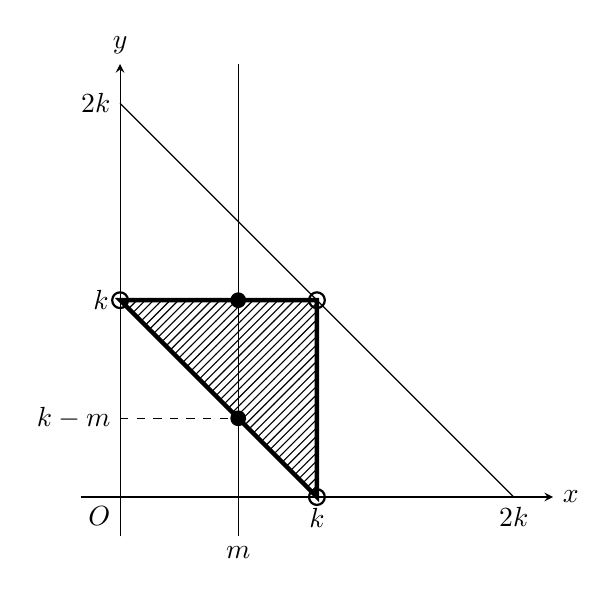
\begin{tikzpicture}
            \draw[ultra thick] (2.5,0) node[below] {$k$} -- (2.5,2.5) -- (0,2.5) node[left] {$k$} -- cycle;
            \fill[gray!80, pattern=north east lines] (2.5,0) -- (2.5,2.5) -- (0,2.5) -- cycle;
            \node[left] at (0, 5) {$2k$};
            \draw[domain=0:5] plot(\x, -\x+5) node[below] {$2k$};
            \draw (1.5,-0.5) node[below] {$m$} -- (1.5,5.5);
            \draw[thick] (2.5,2.5) circle[radius=0.1];
            \draw[thick] (2.5,0) circle[radius=0.1];
            \draw[thick] (0,2.5) circle[radius=0.1];
            \fill (1.5,1) circle[radius=0.1];
            \fill (1.5,2.5) circle[radius=0.1];
            \draw[dashed] (0,1) node[left] {$k-m$} -- (1.5,1);
            \draw[->,>=stealth] (-0.5,0) -- (5.5,0) node[right] {$x$};
            \draw[->,>=stealth] (0,-0.5) -- (0,5.5) node[above] {$y$};
            \node[below left] at (0,0) {$O$};
        \end{tikzpicture}
        \caption{(i)}
    \end{minipage}
    \begin{minipage}{0.49\textwidth}
        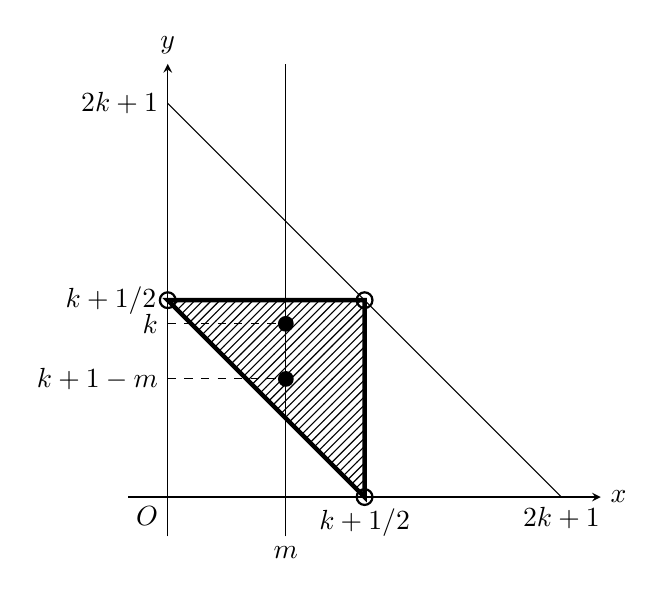
\begin{tikzpicture}
            \draw[ultra thick] (2.5,0) node[below] {$k+1/2$} -- (2.5,2.5) -- (0,2.5) node[left] {$k+1/2$} -- cycle;
            \fill[gray!80, pattern=north east lines] (2.5,0) -- (2.5,2.5) -- (0,2.5) -- cycle;
            \node[left] at (0, 5) {$2k+1$};
            \draw[domain=0:5] plot(\x, -\x+5) node[below] {$2k+1$};
            \draw (1.5,-0.5) node[below] {$m$} -- (1.5,5.5);
            \draw[thick] (2.5,2.5) circle[radius=0.1];
            \draw[thick] (2.5,0) circle[radius=0.1];
            \draw[thick] (0,2.5) circle[radius=0.1];
            \fill (1.5,1.5) circle[radius=0.1];
            \fill (1.5,2.2) circle[radius=0.1];
            \draw[dashed] (0,1.5) node[left] {$k+1-m$} -- (1.5,1.5);
            \draw[dashed] (0,2.2) node[left] {$k$} -- (1.5,2.2);
            \draw[->,>=stealth] (-0.5,0) -- (5.5,0) node[right] {$x$};
            \draw[->,>=stealth] (0,-0.5) -- (0,5.5) node[above] {$y$};
            \node[below left] at (0,0) {$O$};
        \end{tikzpicture}
        \caption{(ii)}
    \end{minipage}
\end{figure}

% ====================

\end{document}
